%%%%%%%%%%%%%%%%%%%%%%%%%%%%%%%%%%%%%%%%%
% CSE 4316/4317 Sprint Report Template
% Version 1.0 (2/18/2018)
% Author: Christopher D. McMurrough
%%%%%%%%%%%%%%%%%%%%%%%%%%%%%%%%%%%%%%%%%

%----------------------------------------------------------------------------------------
%	PACKAGES AND DOCUMENT CONFIGURATIONS
%----------------------------------------------------------------------------------------

\documentclass{article}
\usepackage{siunitx}
\usepackage{graphicx}
\usepackage{amsmath}
\setlength\parindent{0pt}

\usepackage[letterpaper, portrait, margin=1in]{geometry}

%----------------------------------------------------------------------------------------
%	DOCUMENT SECTIONS
%----------------------------------------------------------------------------------------

% report title
\title{Sprint 5 Report \\ CSE 4317}

% author name
\author{Atafo Abure}

% date of assignment submission
\date{February 26th, 2020}

\begin{document}
\maketitle
\begin{center}
\begin{tabular}{l r}

% sprint start date
Sprint start date: & February 10th, 2020 \\

% sprint end date
Sprint end date: & February 24th, 2020 \\

% project title
Project title: & Smart Shutters \\

% team name
Team name: & No SHUT Eye \\

% team members
Partners: 	& Haris Qureshi\\
			& David Nquyen\\
			& Deion Nwaefulu \\
        	& Aditya Rajguru \\
Instructor: & Shawn Gieser
\end{tabular}
\end{center}

% sprint goal
\section{Sprint Goal}
Create DDS Document \\
Set up Bluetooth communication \\
Create Mock Web Server \\

% sprint backlog
\section{Sprint Backlog}
Breakdown of planned tasks assigned to team (work units expressed in days) \\ % work units do not have to be hours, change text accordingly

% ADD OR REMOVE ROWS FROM THE TABLE AS NECESSARY (DO NOT LEAVE BLANK ROWS!)
\begin{tabular}{| p{4in} | >{\centering\arraybackslash} p{1in} | >{\centering\arraybackslash} p{1in} |}
\hline
TASK DESCRIPTION & ESTIMATED WORK & ACTUAL WORK \\ \hline
Start DDS document & 6 & 2 \\ \hline
Mock Web server & 8 & 1 \\ \hline
Set up Bluetooth communication & 14 & 0.5 \\ \hline
\textbf{TOTAL} & \textbf{28}  & \textbf{3.5} \\ \hline
\end{tabular}

\pagebreak

% individual time summary
\section{Individual Time Expenditures}
Summary of tasks performed by the individual (work units expressed in days) \\ % work units do not have to be hours, change text accordingly

% ADD OR REMOVE ROWS FROM THE TABLE AS NECESSARY (DO NOT LEAVE BLANK ROWS!)
% PERCENT COMPLETE DESCRIBES THE STATE OF THE TASK AS OF THE LAST SPRINT DAY (WAS IT FINISHED? IF NOT, APPROXIMATELY HOW "COMPLETE" IS THE TASK)
\begin{tabular}{| p{4in} | >{\centering\arraybackslash} p{1in} | >{\centering\arraybackslash} p{1in} |}
\hline
TASK DESCRIPTION & ACTUAL WORK & PERCENT COMPLETE \\ \hline
DDS Document & 1 & 100\% \\ \hline
Mock Web server & 3 & 90\% \\ \hline
Set up Bluetooth Communications & 5 & 80\% \\ \hline
Create Sprint Presentation & 1 & 100\% \\ \hline
\textbf{TOTAL} & \textbf{10}  & \textbf{-} \\ \hline
\end{tabular}

% burndown chart
\section{Team Burndown Chart}
Burndown chart showing day-to-day progress on sprint tasks. Ideal (baseline) daily effort and actual daily effort of the team are both shown in the figure below.
\begin{figure}[h]
\begin{center}
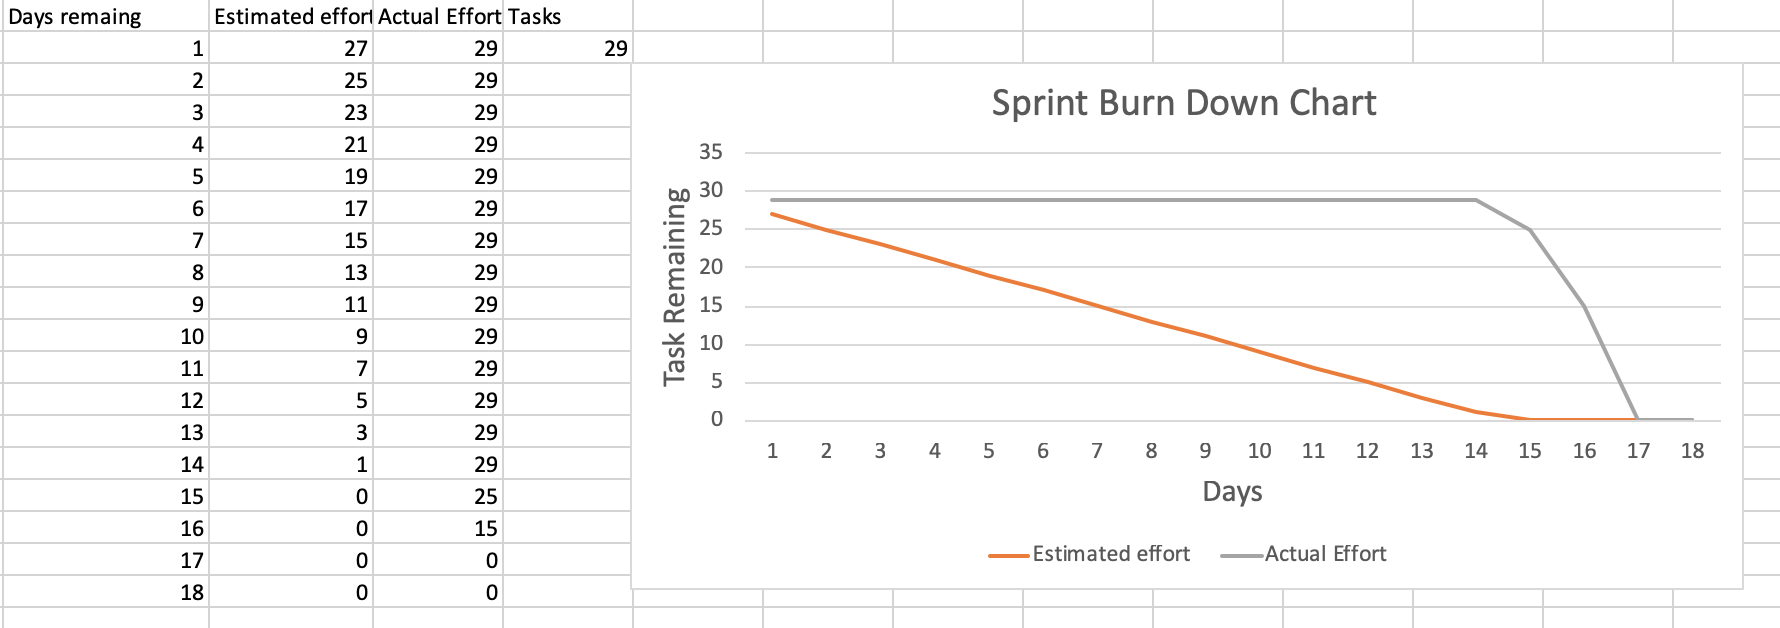
\includegraphics[width=1.0\textwidth]{SprintBurn} % Include the image burndown.png
\end{center}
\end{figure}

\pagebreak

%individual sprint retrospective
\section{Individual Retrospective}
The following lists describe actions (as an individual) that will be started, stopped, or continued during the next sprint to maximize work efficiency. \\

Actions and/or items to \textbf{start} doing in the next sprint (top 3)
\begin{itemize}
\begin{item}
Implement functionality for Add and Remove
\end{item}
\begin{item}
Code Documentation
\end{item}
\begin{item}
Communication between App and Hub
\end{item}
\end{itemize}

Actions and/or items to \textbf{stop} doing in the next sprint (top 3)
\begin{itemize}
\begin{item}
DDS Document
\end{item}
\begin{item}
Web Server
\end{item}
\begin{item}
Bluetooth communication between hub and shutters
\end{item}
\end{itemize}

Actions and/or items to \textbf{continue} doing in the next sprint (top 3)
\begin{itemize}
\begin{item}
Test current functions
\end{item}
\begin{item}
Implement scan function
\end{item}
\begin{item}
Testing with multiple shutters
\end{item}
\end{itemize}

\end{document}